\section{Intra session Coding}
\textit{Consider a source that will send 3 data packets (P1, P2, P3) with n bits each to a destination using RLNC with GF(2). A coded packet CP is generated by a linear combination of the original data packets, i.e.,}

\subsection{Exercise 5: Parameters }
\textit{What is the field size and the generation size in this problem?}\\

The field size is equal to 2 and the generation size is equal to 3. 

\subsection{Exercise 2: Throughput With Network Coding}
\textit{Assuming that the destination has no coded packets at the beginning, what is the probability of a linear combination not being useful? Use the following table that represents the coding coefficients ci of each original packet Pi to identify which case(s) are useful or not. Calculate the probability knowing that each case is equally likely.}\\
\begin{figure}[!h]
  \centering
  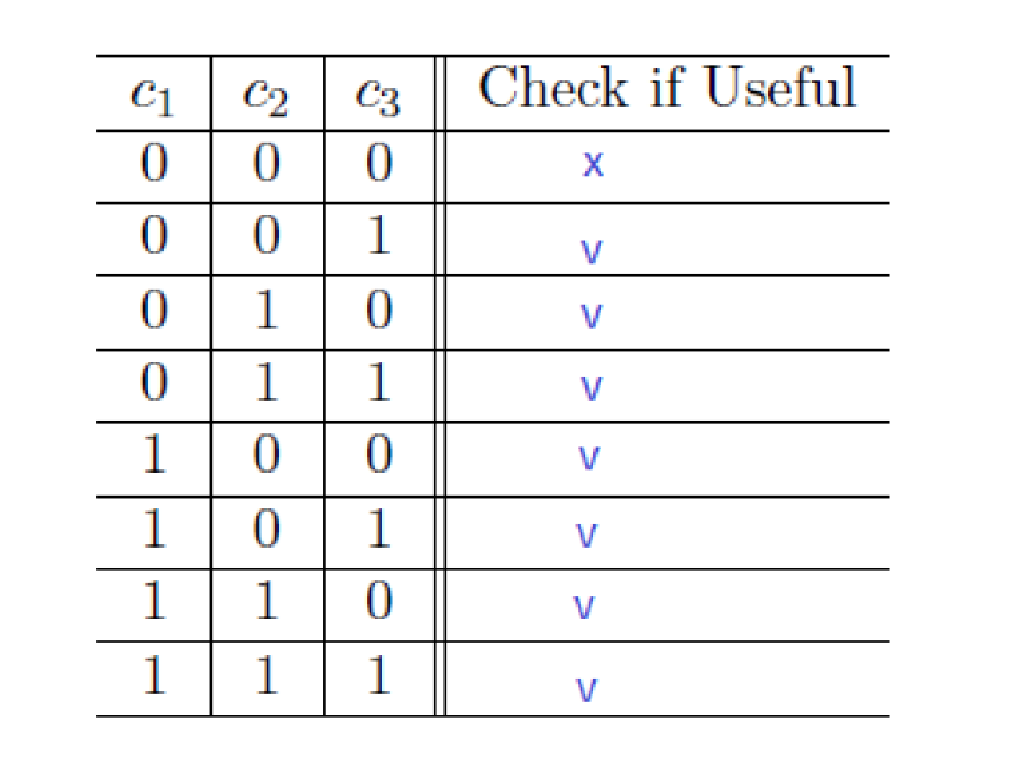
\includegraphics[width=8cm]{Intra_session_1.eps}
  \caption{}
  \label{fig:Intra_session_1}
\end{figure}
In the In \figref{fig:Intra_session_1} the coding coefficient (0, 0, 0) is not useful because the receiver will receive all zeros. So, the probability to receive a useful packet is $P_{useful}=\frac{7}{8}$.\\

\textit{Assuming that one coded packet has arrived to the destination with coding coefficients (0, 1, 1), calculate again the probability of a new incoming coded packet being useful to the receiver. Use the following table for help.}\begin{figure}[!h]
  \centering
  \includegraphics[width=8cm]{Intra_session_2.eps}
  \caption{}
  \label{fig:Intra_session_2}
\end{figure}

In \figref{fig:Intra_session_2} since it has been received the code (0, 1, 1) the probability of having at useful packet at the receiver will be less than before: $P_{useful}=\frac{6}{8}=\frac{3}{4}$.\\

\textit{Assuming that two coded packets have arrived to the destination with coding coefficients (0, 1, 1) and (1, 1, 0), calculate again the probability of a new incoming coded packet being useful to the receiver. Note that this corresponds to the probability of receiving the last useful coded packet before being able to decode. Use the following table for help.}\\
\begin{figure}[!h]
  \centering
  \includegraphics[width=8cm]{Intra_session_3.eps}
  \caption{}
  \label{fig:Intra_session_3}
\end{figure}\\

In \figref{fig:Intra_session_3} the coding (1, 0, 1) is not useful because a linear combination of the two received. So, in the case he probability of having a useful packet at the receiver is $P_{useful}=\frac{4}{8}=\frac{1}{2}$.\\
\FloatBarrier

\subsubsection{What conclusions can you derive from these results?}
After receiving several coded packet the probability of useful packet will not decrease linear due to the linearly dependency among the packed received before. 

\subsubsection{When the generation size is larger, will the probability of receiving the last coded packet before decoding change?}

Since this process can be modelled as a Markov Chain the probability of receiving the last coded packet will not be dependent on the generation size. It will only depend on q.

